\documentclass[11pt, oneside]{article}   	% use "amsart" instead of "article" for AMSLaTeX format
\usepackage{geometry}                		% See geometry.pdf to learn the layout options. There are lots.
\geometry{letterpaper}                   		% ... or a4paper or a5paper or ... 
%\geometry{landscape}                		% Activate for for rotated page geometry
%\usepackage[parfill]{parskip}    		% Activate to begin paragraphs with an empty line rather than an indent
\usepackage{graphicx}				% Use pdf, png, jpg, or eps§ with pdflatex; use eps in DVI mode
								% TeX will automatically convert eps --> pdf in pdflatex		
\usepackage{booktabs}
\usepackage{topcapt}
\usepackage{amssymb}

\title{Theis Equation}
%\author{Hughes, J.D.}
%\date{}							% Activate to display a given date or no date

\begin{document}
\maketitle



\section{Theis Solution}

\begin{figure}[htbp]
   \centering
   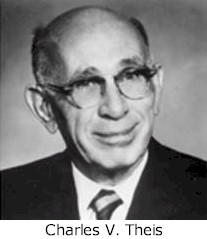
\includegraphics[scale=0.5]{./images/theis_charles_vernon.jpg} % requires the graphicx package
   \label{fig:theis}
\end{figure}

The Theis (1935) equation is used to calculate drawdown for two-dimensional radial groundwater flow to a point source in an infinite, homogeneous aquifer. The Theis equation was derived from heat transfer literature (with the mathematical help of C.I. Lubin) and is defined as:

\begin{equation}
s = \frac{Q}{4 \pi T} W(u)
\end{equation}

\noindent where $s$ is drawdown [L], $Q$ is the pumping rate [L$^3$/T], $T$ is the aquifer transmissivity [L$^2$/T], $u$ is a dimensionless time parameter [unitless], and $W(u)$ is the Well function (exponential integral $E_1$) [unitless]. The exponential integral is available in \texttt{scipy.special} as the \texttt{exp1()} function.

The dimensionless time parameter is defined as:

\begin{equation}
u = \frac{r^2S}{4Tt}
\end{equation}

\noindent where $r$ is the distance from the pumping well to a point where drawdown is observed [L], $S$ is storativity [unitless], and $t$ is the time since pumping began. Storativity is defined as:

\begin{equation}
S = S_s b
\end{equation}

\noindent where $S_s$ is specific storage [1/L] and $b$ is the thickness of the aquifer.

\subsection{Drawdown from a pumping well}

First we will plot drawdown with time at a arbitrary distance from a  pumping well. The relevant parameters are:

% Requires the booktabs if the memoir class is not being used
\begin{table}[htbp]
   \centering
   \topcaption{Aquifer and well parameters} % requires the topcapt package
   \begin{tabular}{@{} lcc @{}} % Column formatting, @{} suppresses leading/trailing space
      \toprule
      Parameter    & Value & Units\\
      \midrule
      x$_{well}$     & 0.     & m \\
      y$_{well}$     & 0.     & m \\
      x$_{obs}$      & 1000.  & m \\
      y$_{obs}$      & 1000.  & m \\
      T              & 0.30   & m$^2$/s \\
      S              & 0.0008 & unitless \\
      Q              & 1.16   &  m$^3$/s \\
      \bottomrule
   \end{tabular}
   %\caption{Remember, \emph{never} use vertical lines in tables.}
   \label{tab:aqparams}
\end{table}

\subsubsection{Exercise 1}

Create a function that calculates the drawdown at a monitor well location. You will also need a function to calculate the distance from the monitor well to the pumping well. Plot drawdown versus time using \texttt{matplotlib}.

\subsubsection{Exercise 2}

Make new functions from your existing drawdown and distance functions to calculate the drawdown for a square area with a fixed cell size ($\Delta x = \Delta y$) and a pumping well in the center of the area. Your functions should be able to work with two-dimensional \texttt{numpy} arrays and return a \texttt{numpy} drawdown array that can be plotted with \texttt{matplotlib}. Use an odd number of rows and columns (rows = columns) so that the pumping well is located in center of the area.





\end{document}  